%%%%%%%%%%%%%%%%%%%%% chapter.tex %%%%%%%%%%%%%%%%%%%%%%%%%%%%%%%%%
%
% sample chapter
%
% Use this file as a template for your own input.
%
%%%%%%%%%%%%%%%%%%%%%%%% Springer-Verlag %%%%%%%%%%%%%%%%%%%%%%%%%%
%\motto{Use the template \emph{chapter.tex} to style the various elements of your chapter content.}
\chapter{Introduction}
\label{intro} 

\abstract*{The increasing penetration of mobile-connected devices and the emergence of numerous data-hungry mobile applications has created a wide range of business opportunities for mobile network operators and service providers. Meanwhile, this growth is placing a greater pressure on the capacity that the Radio Access Networks (RANs) have to provide. This chapter begins with a review of technical challenges that motivate developments of cost-effective solutions to improve the capacity of RANs. The technology which utilizes the unlicensed frequency bands in Long-Term Evolution (LTE), namely U-LTE, is singled out as the most promising solution. Benefits and obstacles of this technology are then presented. Next, three typical forms of U-LTE including LTE-U, LAA-LTE, and MulteFire are explained. Concerns on the interactions between U-LTE and Wi-Fi in radio channel access and their coexistence are discussed in detail. Finally, key requirements for the coexistence of U-LTE and Wi-Fi are summarized.}  

The increasing penetration of mobile-connected devices and the emergence of numerous data-hungry mobile applications has created a wide range of business opportunities for mobile network operators and service providers. Meanwhile, this growth is placing a greater pressure on the capacity that the Radio Access Networks (RANs) have to provide. This chapter begins with a review of technical challenges that motivate developments of cost-effective solutions to improve the capacity of RANs. The technology which utilizes the unlicensed frequency bands in Long-Term Evolution (LTE), namely U-LTE, is singled out as the most promising solution. Benefits and obstacles of this technology are then presented. Next, three typical forms of U-LTE including LTE-U, LAA-LTE, and MulteFire are explained. Concerns on the interactions between U-LTE and Wi-Fi in radio channel access and their coexistence are discussed in detail. Finally, key requirements for the coexistence of U-LTE and Wi-Fi are summarized.


\section{Motivations and Concepts of U-LTE}
\label{lte-motiv}

Global mobile traffic is expected to increase nearly tenfold between 2014 and 2020 due to the increasing number of mobile-connected devices and the explosion of data-hungry mobile applications \cite{cisco_mobile_traffic_2015}. The expected growth in traffic is shown in detail in Fig. \ref{figs:global-mobile-data-traffic-2015-2020}, where the $3.7$ exabytes per month seen in 2015 is forecast to grown at a compound annual growth rate of 53\%, reaching $30.6$ exabytes per month by 2020. 
\begin{figure}[!ht]
	\centering
	\includegraphics[width=\textwidth]{figs/global-mobile-data-traffic-2015-2020}
	\caption{Global mobile data traffic from 2015-2020 \cite{cisco_mobile_traffic_2015}.}
	\label{figs:global-mobile-data-traffic-2015-2020}
\end{figure}
Pushing traffic towards the network capacity quickly deteriorates the Quality of Service (QoS) perceived by the users. As a result, increasing the capacity of their Radio Access Network (RAN) is one of the top-priority action plans of mobile service providers. Purchasing additional licensed spectrum is a straight-forward solution to this but radio spectrum is very much limited and increasingly expensive. Furthermore, mobile operators are at the same time challenged by the ``revenue gap'', i.e., the exponential increase in mobile traffic does not generate sufficient additional revenues which would be required for upgrading their RANs. This circumstance has fostered interest in cost-effective solutions to increase RAN capacity. Mobile data off-loading and Long-Term Evolution (LTE) in unlicensed bands (U-LTE) are among the most promising solutions.

Mobile data offloading is the use of a complementary wireless technology to transport data originally flowing through the cellular mobile network. Wi-Fi offloading and Device-to-Device (D2D) communications are the two main data offload techniques. Rules determining when and how the mobile offloading actions are triggered are set by either mobile subscribers or network operators. For the subscribers, data offloading helps them to exploit the availability of higher bandwidth data service at lower costs. For the operators, the most obvious benefit of this kind of approach is the mitigation of cellular mobile network load and thus congestion. Besides, shifting data to a complementary wireless technology leads to a number of other improvements including an overall increase in network throughput, a reduction of content delivery time, the extension of network coverage and increase of network availability, and better energy efficiency. Unfortunately, these benefits come with a number of challenges related to infrastructure coordination, network/technology hand-overs, service continuity, pricing, business models, and lack of existing standards. 

Recently, U-LTE has appeared as the most promising approach to enhance RAN capacity and address the revenue gap in mobile networks. The original idea of LTE-U is fairly straightforward: By definition, it is an LTE technology that puts cellular signals into the unlicensed spectrum with the support of existing LTE features including Supplemental Downlink (SDL, proposed in LTE Release 9 and later) and Carrier Aggregation (CA, proposed in LTE Release 10 and later).  As mentioned, mobile operators are facing a great pressure on capacity and cost. If LTE can exploit the unlicensed band (where IEEE 802.11/Wi-Fi and other radio systems are using), then it will obtain a considerable additional capacity at a minimal cost. U-LTE can be used to boost downlink or both uplink and downlink of LTE networks, as illustrated in Fig. \ref{figs:U-LTE-use_model}.
\begin{figure}[!ht]
	\centering
	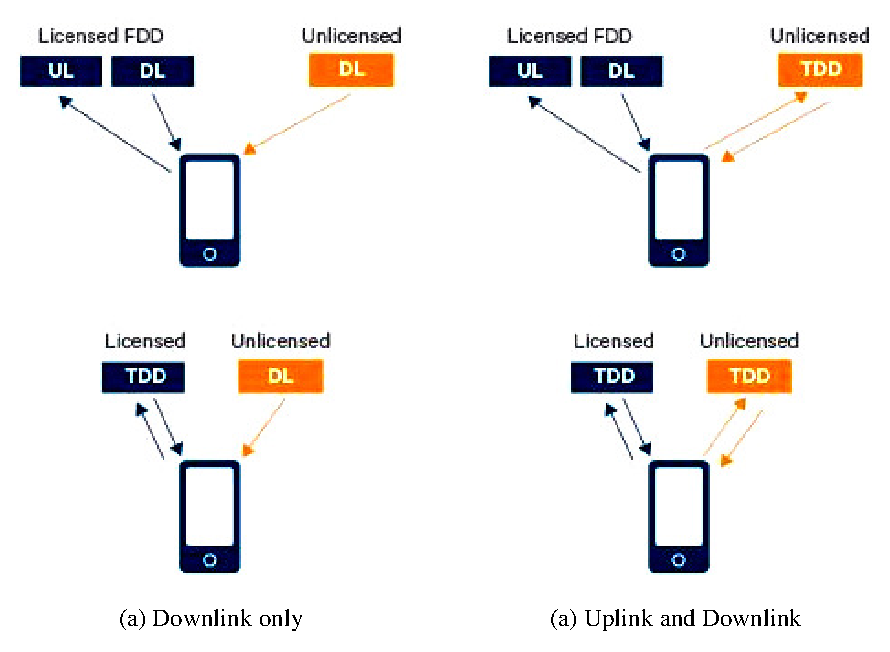
\includegraphics[width=0.75\textwidth]{figs/U-LTE-use_model}
	\caption{Use cases of U-LTE.}
	\label{figs:U-LTE-use_model}
\end{figure}

Historically, U-LTE was originally proposed and officially announced by Qualcomm in 2013 \cite{Qualcomm-U-LTE-2013}. Currently, it focuses on $500$ MHz of spectrum available in the $5$ GHz band. Specifically, according to the proposal from Qualcomm, U-LTE is to use the U-NII-3 part of the $5$ GHz band, which has highest allowed Equivalent Isotropically Radiated Power (EIRP). While in the $2.4$ GHz band, regulatory bodies limit EIRP to $100$ mW (in Europe) or $200$ mW (in United States), the U-NII-3 enjoys the rights to go as high as $1000$ mW outdoors.

\section{Benefits and Obstacles of U-LTE}
\label{lte-ben}
U-LTE is expected to offer numerous benefits to mobile network operators, service providers, and consumers. Free access to the unlicensed spectrum provides additional capacity to the network at a minimal cost compared to purchasing licensed spectrum allocations. Therefore, U-LTE appears to be a very inexpensive way to meet the future traffic growth. U-LTE will give operators the option to make use of unlicensed spectrum within a unified network, offering potential operational cost savings, improving spectral efficiency, and providing a better user experience. Compared to the Wi-Fi offloading technology, U-LTE has the potential to offer significantly better coverage and higher spectral efficiency while allowing seamless flow of data across licensed and unlicensed channels in a single core network. U-LTE could also take advantage of the robust security features which are already in place in LTE networks, rather than relying on external or complementary networks. Finally, Wi-Fi offloading leads to less traffic on mobile networks and thus may result in revenue losses in data services.  Since U-LTE could be managed through a single core network, it could provide an incremental ability for mobile service providers to directly bill for data usage.

Despite the obvious benefits of U-LTE, there are a number of substantial obstacles. First, even though U-LTE is not charged for the use of unlicensed spectrum, compared to Wi-Fi, its network deployment could be more expensive. The LTE chipset itself is several times more expensive than that of Wi-Fi (a few tens of dollars compared to a few dollars or less than one dollar). LTE base stations and other network devices are likely to cost substantially more than the required Wi-Fi access points to service the same area in the unlicensed bands.  Also, LTE operators need to deploy and maintain expensive back-haul links between base stations and from the base station to the core network. Being an LTE technology, U-LTE will work only with LTE-capable devices while there have been many more devices that feature Wi-Fi connectivity than LTE. Wi-Fi is nearly always integrated into laptops, tablets, cameras, and other connected consumer devices. Additionally, from technical perspectives, the premium features provided by U-LTE (e.g., seamless voice and data roaming) may not prove sufficiently more valuable than those offered by emerging Wi-Fi technologies such as Hotspot 2.0, so-called Wi-Fi Certified Passpoint, which is a new standard for public-access Wi-Fi that enables seamless roaming among Wi-Fi networks and between Wi-Fi and cellular networks. Finally, the biggest challenge of U-LTE is its coexistence with other radio networks operating in the same frequency bands. 

\section{Three Types of U-LTE}
\label{lte-types}
There are three different flavors of U-LTE currently under development: LTE unlicensed (LTE-U), Licensed Assisted Access LTE (LAA-LTE), and MulteFire. The first two flavors require ``anchoring licensed spectrum'', i.e., they operate primarily in licensed spectrum and opportunistically exploit access to the unlicensed spectrum for an additional bandwidth boost. Devices are still anchored in licensed spectrum for LTE management/control signaling and high QoS data while using the unlicensed spectrum for only best-effort or delay-tolerant data. The third flavor is developed by Qualcomm and requires no licensed spectrum at all, therefore, it is often referred to as stand-alone U-LTE. MulteFire is designed for indoor use and deployments by enterprises, cable companies and other service providers without ownership of expensive bandwidth licenses. However, at the present time, there are very few technical details available about MulteFire.


\subsection{LTE-U}
LTE-U is the simplest form of U-LTE and requires only minor modifications in LTE protocol stack. Therefore, it can quickly facilitate pre-standard equipment manufacturing and deployment. LTE-U first attempts to select a clear channel to access. If no clear channel is found, it will employ Carrier-Sensing Adaptive Transmission (CSAT), which is a Time-Division Multiplex (TDM) coexistence mechanism based on medium sensing. The CSAT mechanism is depicted in in Fig. \ref{figs:LTE-U}.
\begin{figure}[!ht]
	\centering
	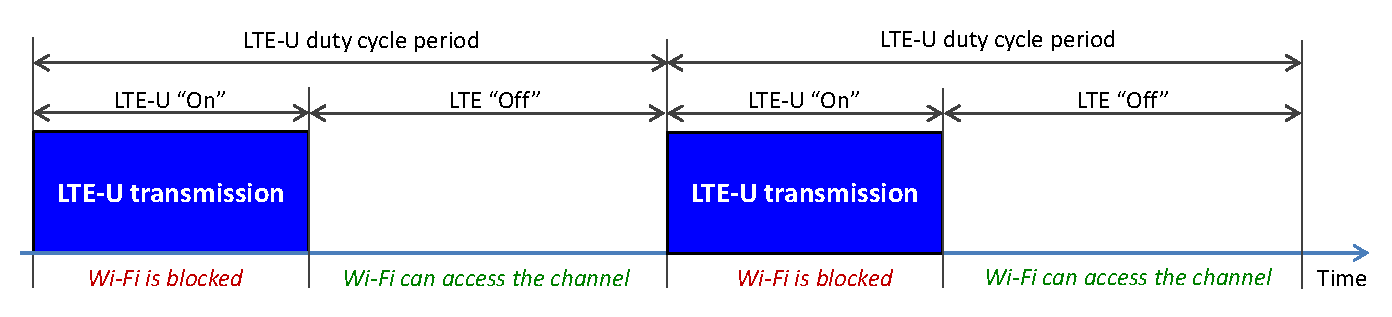
\includegraphics[width=\textwidth]{figs/LTE-U}
	\caption{Duty-cycling mechanism employed by LTE-U.}
	\label{figs:LTE-U}
\end{figure}
CSAT employs duty-cycling, which enforces the TDM cycle on other users of the channel, instead of LBT mechanism.  In particular, CSAT defines a time cycle where the base station transmits in a fraction of the cycle and then gates off in the remaining duration. Compared to LBT or CSMA, the base station senses the medium for a longer duration (around $10$s of milliseconds to $200$ milliseconds) and according to the observed medium activities the algorithm gates off LTE transmission proportionally.  The duty cycle of transmission versus gating off is dictated by the sensed medium activity of neighboring RANs. The TDM cycle can be set to a few tens or hundreds of millisecond, which can effectively accommodate the activation/de-activation procedures while controlling the data transmission delay. An important observation from Fig. \ref{figs:LTE-U} is that during the LTE ``on'' period, Wi-Fi is blocked by LTE-U transmissions. During the LTE ``off'' period, Wi-Fi will detect that the channel is free and can schedule its transmissions following its CSMA-CA protocol.

LTE-U is only applicable in areas where there are no strict LBT requirements for operations in unlicensed bands (e.g., US, Korea, and China). It is a non-standard version of U-LTE, being developed outside of the 3GPP standards process. LTE-U is supported by the LTE-U Forum formed in 2014 by Verizon in cooperation with Alcatel-Lucent, Ericsson, Qualcomm Technologies Inc. (a subsidiary of Qualcomm Incorporated), and Samsung.

\subsection{LAA-LTE}
In many regions (e.g., Europe, Japan, and India) there exist regulations for accessing the unlicensed spectrum that require equipment to periodically check for the presence of other occupants in the channel, so-called LBT. LAA-LTE is designed for use in such areas, but also for global use. It requires a number of modifications so that LTE transmissions can meet regulatory requirements in LBT regions. Similar to LTE-U, LAA-LTE first tries to choose the cleanest channel available, based on Wi-Fi and LTE measurements. In the event that no clean channel is available, a LBT algorithm is used to compete for the medium with other RANs. For LBT, different mechanisms for frame-based equipment (FBE) and load-based equipment (LBE) have been specified in \cite{LBT-ETSI-2014}. Details of these types of the devices and the applicable mechanisms are presented in Chapter \ref{sec:LBT-overview}.

Assuming that LBE LBT is employed for LAA-LTE, before transmission, a clear channel assessment  (CCA) using and energy detect (ED) threshold is performed. If the channel is clear during a CCA slot ($20$ microseconds or longer), transmission is started immediately. Otherwise, and extended CCA (ECCA) is performed. If the channel is clear during $N$ CCA slots, transmission is started immediately where $N$ is a random integer uniformly distributed from $1$ to $q$, and $q \in \{4,5,...,32\}$ is a pre-determined constant. The total time to occupy the channel without CCA is limited to $(13/32)q$ milliseconds (e.g., $13$ milliseconds when $q$ is $32$). Two simplified scenarios with LAA-LTE (employing LBE-based LBT) and Wi-Fi systems operating in the same channel are illustrated in Fig. \ref{figs:LAA-LTE}. 
\begin{figure}[!ht]
	\centering
	\includegraphics[width=0.9\columnwidth]{figs/LAA-LTE}
	\caption{CCA and ECCA mechanisms employed by LAA-LTE.}
	\label{figs:LAA-LTE}
\end{figure}
In the first scenario, the LAA-LTE system, upon having data frames to send, performs CCA and then ECCA (with $N=7$) since there is an ongoing Wi-Fi transmission. The ECCA procedure is frozen and then resumed when another Wi-Fi transmission takes place and then completes, respectively. The LAA-LTE system finally transmits its frames once its ECCA counter reaches zero. In the second scenario, the Wi-Fi system, upon having data frames to send, performs CCA and then back-off procedure (with $\mathrm{BI_{slots}} = 7$) since there is an ongoing LAA-LTE transmission. The back-off procedure is frozen and resumed when another LAA-LTE transmission takes place. The Wi-Fi system finally transmits its frames once back-off counter reaches zero.

Since LTE was originally designed for licensed spectrum and a centralized management (i.e., network-controlled) model, it is generally an ``always-on'' technology. As a result, adapting to LBT is a marked change for the LTE protocol. Compared to LTE-U, which is downlink-only in the unlicensed bands, LAA-LTE may be used to support bi-directional traffic in unlicensed bands. LAA-LTE is currently actively supported by 3GPP and is included in 3GPP LTE Release 13. T-Mobile USA and Verizon Wireless have indicated their interests in deploying pre-standard LAA-LTE systems for evaluations and commercial services in 2016.



\subsection{MulteFire}
At this time there are very few technical details available about MulteFire. It is unknown which MAC protocols or coexistence mechanisms are employed in this type of U-LTE. Also, since licensed frequency is not used for LTE network management and control signaling, as opposed to the conventional LTE and the other two variants of U-LTE (i.e., LTE-U and LAA-LTE) that are license anchored, MulteFire may lose all advantages of native LTE technologies. It is expected that MulteFire will be less efficient than LTE-U and LAA-LTE and therefore its achievable performance/efficiency may be just marginally better than that of Wi-Fi. Then the question on the applicability of MulteFire needs to be answered.


\section{Coexistence of U-LTE and Wi-Fi}
\label{coexist}
It is well known that multiple radio communications technologies operating in a common frequency band will negatively affect each other if respectful coexistence mechanisms are not employed. As a result, despite the fact that U-LTE can offer various benefits, its coexistence with Wi-Fi and other radio systems that operate in the $5$ GHz frequency band is the biggest concern. In specific, it is believed that U-LTE may considerably interfere with Wi-Fi systems and/or grasp more radio resources when they operate in the same frequency band due to the following:
\begin{itemize}
\item \textit{First}, LTE was originally designed to work in its own licensed frequency band rather than to coexist with other radio access technologies in a shared band. LTE employs Orthogonal Frequency-Division Multiple Access (OFDMA) and transmits almost continuously without requiring or implementing any mechanism for spectrum sharing. Wi-Fi, on the other hand, employs a Listen-Before-Talk (LBT) medium access strategy.  In fact, the Wi-Fi LBT protocol includes a few key additional features that go beyond the LBT requirements specified by European Telecommunications Standards Institute (ETSI) \cite{LBT-ETSI-2014}. As a result, U-LTE might overwhelm Wi-Fi neighbors with its aggressive transmission profile, if no relevant coexistence measure is implemented.

\item \textit{Second}, the typical duration of transmission for LTE and Wi-Fi are not the same. LTE, due to its basic protocol design and scheduled nature, generally transmits long frames (i.e., multiple ms), whereas a large percentage of Wi-Fi frames are sub-millisecond in duration. For this reason, equitable access to the medium, evaluated in terms of how often a technology is able to start a transmission, does not necessarily translate into equitable airtime.

\item \textit{Third}, a license-anchored system (LTE-U or LAA-LTE) operates simultaneously in licensed and unlicensed bands.  Thus such systems can dynamically move traffic between the bands on a granular basis (e.g., per-user and per-flow). As a result, such a system is inherently less sensitive to collisions and congestion in the unlicensed bands than a system operating solely in the unlicensed spectrum bands.  This reduced sensitivity to the issues which arise from coexistence may reduce the incentive for a license-anchored system to develop effective coexistence mechanisms.
\end{itemize}

In fact, U-LTE is still a nascent LTE technology with many technical details to be determined. Proponents of U-LTE include Qualcomm, Ericsson, Alcatel-Lucent, Huawei, LTE-U Forum, 3rd Generation Partnership Project (3GPP), Verizon Wireless, T-Mobile US, etc. At the same time, CableLabs, Google, Wi-Fi Alliance, The Institute of Electrical and Electronics Engineers Standards Association (IEEE-SA), and many Wi-Fi interested companies, are participating in and following closely the development of U-LTE technology. These organizations have been expressing their concerns and the critical need for strong coexistence between U-LTE and Wi-Fi to ensure responsible and fair use of the unlicensed spectrum. As a result, various studies on the coexistence of U-LTE and Wi-Fi have been carried out by both industry and academia. Besides, a number of reports and comments related to this concern have been filed with the Federal Communications Commission (FCC).


\section{Requirements of U-LTE Coexistence Mechanisms}
\label{reqs}
Even though the unlicensed bands may be used by anyone, there is a series of government guidelines and regulations which must be followed. These guidelines and regulations aim to ensure that different radio systems operating in the same frequency bands are good neighbors to each other. In particular, for coexistence with Wi-Fi, at minimum U-LTE must satisfy local regulations such as the maximum transmission power in specific bands and the avoidance of bands dedicated to protected services. Furthermore, an U-LTE system should not cause any higher interference to a neighboring Wi-Fi system than a typical Wi-Fi system operating on the same channel. In other words, the impact of a U-LTE device to Wi-Fi devices (in terms of collision rate and probability of successful channel access) should be similar to that caused by a typical Wi-Fi device. These requirements ask for inclusions of a number of new features in LTE. For example, U-LTE should select a carrier which is least occupied in the area and should dynamically change operating frequency to avoid conflict with protected systems, such as radar. It should also apply LBT or Clear Channel Assessment (CCA) techniques to check that a channel is free before making a transmission. Exactly how these decisions are made will be key aspects of U-LTE system designs.


\section{Structure of This Brief}

This Springer Brief is divided into seven chapters. This introductory chapter has provided an overview of the emerging U-LTE technology and its accompanying motivations, concepts, benefits, and challenges. The technical concerns surrounding the coexistence of this new LTE technology and the existing Wi-Fi networks operating in the $5$ GHz unlicensed frequency bands has also been described. The remainder of this brief is organized as follows: 

For background knowledge, Chapter \ref{sec:LBT-overview} provides an overview on radio spectrum and related management/allocation concerns in the $5$ GHz unlicensed frequency band. It also summarizes a number of the key requirements and regulations specified by the European Telecommunications Standards Institute (ETSI) and the Federal Communications Commission (FCC) applying to radio channels, operating channel selection, transmission power, and channel access rules. These technical details are the baselines to be followed when designing medium access control protocols for U-LTE and any other technologies which are designed for shared bands.

Chapter \ref{overview-lte} presents a high-level overview of LTE-Advanced (LTE-A) networks and associated technologies to form a basis for discussion of the co-existence issues that exist for unlicensed LTE and Wi-Fi. Understanding the underlying architecture and protocols employed in LTE-A will provide readers a comparative framework to grasp how, and at what levels, LTE and Wi-Fi networks may interact and interfere with each other, and form a greater understanding of the challenges to be address in designing coexistence mechanisms.

Furthering the basis for framing the potential problems with U-LTE/Wi-Fi coexistence, Chapter \ref{overview-wifi} focuses on Wi-Fi technology, beginning with an overview of the evolution of IEEE 802.11/Wi-Fi. Both existing Wi-Fi generations as well as the next generation of IEEE 802.11/Wi-Fi currently under development are presented. The majority of this chapter provides the underlying ideas and detailed mechanisms of the CSMA/CA MAC protocol used in Wi-Fi. Important observations on how CSMA/CA senses and occupies the radio medium when the LTE network is operating in vicinity are highlighted.

Chapter \ref{survey} provides a current literature survey to present a big picture of the research activities related to the coexistence of U-LTE and Wi-Fi technologies. The following questions are addressed in this chapter: 
\begin{itemize}
\item What issues arise from simultaneous operation of LTE and Wi-Fi in the same spectrum bands? 
\item Which technology is affected the most. 
\item Which factors determine the impacts of U-LTE to Wi-Fi. 
\end{itemize}Finally, the chapter identifies the strengths and weaknesses of existing solutions and suggests potential strategies to improve the performance of these two technologies.

In Chapter \ref{intro-NALT}, a network-aware adaptive Listen-Before-Talk mechanism (NALT) proposed for U-LTE is presented. To promote effective coexistence in terms of channel occupancy time, NALT passively monitors both channel conditions and usage activity to maximize its own transmission opportunities while respecting fair sharing of the channel, in a way that is transparent to incumbent Wi-Fi devices. Simulation results are presented, demonstrating the effectiveness of NALT in providing proportional fair sharing among contending LAA-LTE and Wi-Fi devices.

Finally, Chapter \ref{open-research} ends this Springer Brief by addressing a number of research issues and associated potential research directions. Potential solutions to the issues identified are also discussed. Most of the solutions suggest the cooperation of LTE and Wi-Fi so that they could have a better understanding of each other when operating in the same area using the same radio frequency band. This understanding is used to have more vigilant actions that help to avoid aggressive channel access that could corrupt on-going transmissions and to design relevant protocols for a fair spectrum sharing.


%%%%%%%%%%%%%%%%%%%%%%%% referenc.tex %%%%%%%%%%%%%%%%%%%%%%%%%%%%%%
% sample references
% %
% Use this file as a template for your own input.
%
%%%%%%%%%%%%%%%%%%%%%%%% Springer-Verlag %%%%%%%%%%%%%%%%%%%%%%%%%%
%%
%% BibTeX users please use
%% \bibliographystyle{}
%% \bibliography{}

\begin{thebibliography}{99.}%
\bibitem{cisco_mobile_traffic_2015}``Cisco visual networking index: Global mobile data traffic forecast update 2014-2019,'' white paper, Cisco, 2015.	
	
\bibitem{Qualcomm-U-LTE-2013}``Extending {LTE} advanced to unlicensed spectrum,'' white paper, Qualcomm Inc., Dec. 2013.

\bibitem{LBT-ETSI-2014} \emph{ETSI EN 301 893 V1.7.2 (2014-07): Broadband radio access networks (BRAN);	5 GHz high performance RLAN; Harmonized EN covering the essential requirements of article 3.2 of the R\&TTE Directive}, European Telecommunications Standards Institute Std., 2014.	
\end{thebibliography}
